\begin{prob}

    An \emph{edge weighted graph} $G = (V,E,\omega)$ is a graph along with
        a function $\omega : E \to \mathbb R$ which assigns a weight to every
        edge in the graph. One of the uses of edges weights is to encode dissimilarities.
        That is, the greater the weight of an edge, the more dissimilar the nodes
        at either end.

        A natural task involving weighted graphs is to \emph{cluster} the nodes
        of the graph into groups such that nodes in the same group are similar to
        one another while two nodes in different groups are dissimilar.

        Here is a simple way of clustering a weighted, undirected graph $G =
        (V,E,\omega)$.  Given a real number $t$, place two nodes $u$ and $v$ in
        the same cluster if (and only if) there is a path between $u$ and $v$
        along which every edge has weight $\leq t$. For instance, consider the graph below:

        \noindent
        \begin{minipage}{0.5\textwidth}
        \centering
        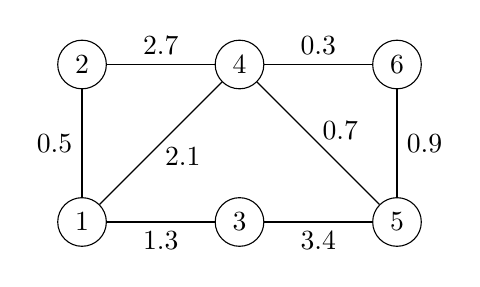
\begin{tikzpicture}
            \node[draw, circle] (n1) at (0,0) {1};
            \node[draw, circle] (n2) at (0,2) {2};
            \node[draw, circle] (n3) at (2,0) {3};
            \node[draw, circle] (n4) at (2,2) {4};
            \node[draw, circle] (n5) at (4,0) {5};
            \node[draw, circle] (n6) at (4,2) {6};

            \draw (n3) -- node[below] {3.4} (n5);
            \draw (n1) -- node[below] {1.3} (n3);
            \draw (n2) -- node[above] {2.7} (n4);
            \draw (n4) -- node[above] {0.3} (n6);
            \draw (n6) -- node[right] {0.9} (n5);
            \draw (n1) -- node[left] {0.5} (n2);
            \draw (n4) -- node[above right=-.2em] {0.7} (n5);
            \draw (n4) -- node[below right=-.2em] {2.1} (n1);
        \end{tikzpicture}
        \end{minipage}%
        \begin{minipage}{0.5\textwidth}
        If $t = 1$, there are three clusters: $\{1, 2\}$, $\{4, 5, 6\}$ and $\{3\}$.
        If $t = 2$, there are two clusters: $\{1, 2, 3\}$ and $\{4, 5, 6\}$.
        And if $t = 3$, there is one cluster containing all of the nodes.
        \end{minipage}

        Design an algorithm which returns the clusters given an input graph, a weight function, weights, and a threshold t.
        Your algorithm should take $\Theta(V + E)$ time. To receive full credit, your algorithm should not modify the graph or create a copy of it.
        Provide pseudocode (or Python).

    \begin{soln}
        \inputminted{python}{\thisdir/include/cluster_answer.py}
    \end{soln}

\end{prob}
